\documentclass[12pt,a4paper]{article}

\usepackage[a4paper,text={16.5cm,25.2cm},centering]{geometry}
\usepackage{lmodern}
\usepackage{amssymb,amsmath}
\usepackage{bm}
\usepackage{graphicx}
\usepackage{microtype}
\usepackage{hyperref}
\setlength{\parindent}{0pt}
\setlength{\parskip}{1.2ex}

\hypersetup
       {   pdfauthor = { Shalin Patel },
           pdftitle={ Generating Data },
           colorlinks=TRUE,
           linkcolor=black,
           citecolor=blue,
           urlcolor=blue
       }

\title{ Generating Data }

\author{ Shalin Patel }


\usepackage{upquote}
\usepackage{listings}
\usepackage{xcolor}
\lstset{
    basicstyle=\ttfamily\footnotesize,
    upquote=true,
    breaklines=true,
    breakindent=0pt,
    keepspaces=true,
    showspaces=false,
    columns=fullflexible,
    showtabs=false,
    showstringspaces=false,
    escapeinside={(*@}{@*)},
    extendedchars=true,
}
\newcommand{\HLJLt}[1]{#1}
\newcommand{\HLJLw}[1]{#1}
\newcommand{\HLJLe}[1]{#1}
\newcommand{\HLJLeB}[1]{#1}
\newcommand{\HLJLo}[1]{#1}
\newcommand{\HLJLk}[1]{\textcolor[RGB]{148,91,176}{\textbf{#1}}}
\newcommand{\HLJLkc}[1]{\textcolor[RGB]{59,151,46}{\textit{#1}}}
\newcommand{\HLJLkd}[1]{\textcolor[RGB]{214,102,97}{\textit{#1}}}
\newcommand{\HLJLkn}[1]{\textcolor[RGB]{148,91,176}{\textbf{#1}}}
\newcommand{\HLJLkp}[1]{\textcolor[RGB]{148,91,176}{\textbf{#1}}}
\newcommand{\HLJLkr}[1]{\textcolor[RGB]{148,91,176}{\textbf{#1}}}
\newcommand{\HLJLkt}[1]{\textcolor[RGB]{148,91,176}{\textbf{#1}}}
\newcommand{\HLJLn}[1]{#1}
\newcommand{\HLJLna}[1]{#1}
\newcommand{\HLJLnb}[1]{#1}
\newcommand{\HLJLnbp}[1]{#1}
\newcommand{\HLJLnc}[1]{#1}
\newcommand{\HLJLncB}[1]{#1}
\newcommand{\HLJLnd}[1]{\textcolor[RGB]{214,102,97}{#1}}
\newcommand{\HLJLne}[1]{#1}
\newcommand{\HLJLneB}[1]{#1}
\newcommand{\HLJLnf}[1]{\textcolor[RGB]{66,102,213}{#1}}
\newcommand{\HLJLnfm}[1]{\textcolor[RGB]{66,102,213}{#1}}
\newcommand{\HLJLnp}[1]{#1}
\newcommand{\HLJLnl}[1]{#1}
\newcommand{\HLJLnn}[1]{#1}
\newcommand{\HLJLno}[1]{#1}
\newcommand{\HLJLnt}[1]{#1}
\newcommand{\HLJLnv}[1]{#1}
\newcommand{\HLJLnvc}[1]{#1}
\newcommand{\HLJLnvg}[1]{#1}
\newcommand{\HLJLnvi}[1]{#1}
\newcommand{\HLJLnvm}[1]{#1}
\newcommand{\HLJLl}[1]{#1}
\newcommand{\HLJLld}[1]{\textcolor[RGB]{148,91,176}{\textit{#1}}}
\newcommand{\HLJLs}[1]{\textcolor[RGB]{201,61,57}{#1}}
\newcommand{\HLJLsa}[1]{\textcolor[RGB]{201,61,57}{#1}}
\newcommand{\HLJLsb}[1]{\textcolor[RGB]{201,61,57}{#1}}
\newcommand{\HLJLsc}[1]{\textcolor[RGB]{201,61,57}{#1}}
\newcommand{\HLJLsd}[1]{\textcolor[RGB]{201,61,57}{#1}}
\newcommand{\HLJLsdB}[1]{\textcolor[RGB]{201,61,57}{#1}}
\newcommand{\HLJLsdC}[1]{\textcolor[RGB]{201,61,57}{#1}}
\newcommand{\HLJLse}[1]{\textcolor[RGB]{59,151,46}{#1}}
\newcommand{\HLJLsh}[1]{\textcolor[RGB]{201,61,57}{#1}}
\newcommand{\HLJLsi}[1]{#1}
\newcommand{\HLJLso}[1]{\textcolor[RGB]{201,61,57}{#1}}
\newcommand{\HLJLsr}[1]{\textcolor[RGB]{201,61,57}{#1}}
\newcommand{\HLJLss}[1]{\textcolor[RGB]{201,61,57}{#1}}
\newcommand{\HLJLssB}[1]{\textcolor[RGB]{201,61,57}{#1}}
\newcommand{\HLJLnB}[1]{\textcolor[RGB]{59,151,46}{#1}}
\newcommand{\HLJLnbB}[1]{\textcolor[RGB]{59,151,46}{#1}}
\newcommand{\HLJLnfB}[1]{\textcolor[RGB]{59,151,46}{#1}}
\newcommand{\HLJLnh}[1]{\textcolor[RGB]{59,151,46}{#1}}
\newcommand{\HLJLni}[1]{\textcolor[RGB]{59,151,46}{#1}}
\newcommand{\HLJLnil}[1]{\textcolor[RGB]{59,151,46}{#1}}
\newcommand{\HLJLnoB}[1]{\textcolor[RGB]{59,151,46}{#1}}
\newcommand{\HLJLoB}[1]{\textcolor[RGB]{102,102,102}{\textbf{#1}}}
\newcommand{\HLJLow}[1]{\textcolor[RGB]{102,102,102}{\textbf{#1}}}
\newcommand{\HLJLp}[1]{#1}
\newcommand{\HLJLc}[1]{\textcolor[RGB]{153,153,119}{\textit{#1}}}
\newcommand{\HLJLch}[1]{\textcolor[RGB]{153,153,119}{\textit{#1}}}
\newcommand{\HLJLcm}[1]{\textcolor[RGB]{153,153,119}{\textit{#1}}}
\newcommand{\HLJLcp}[1]{\textcolor[RGB]{153,153,119}{\textit{#1}}}
\newcommand{\HLJLcpB}[1]{\textcolor[RGB]{153,153,119}{\textit{#1}}}
\newcommand{\HLJLcs}[1]{\textcolor[RGB]{153,153,119}{\textit{#1}}}
\newcommand{\HLJLcsB}[1]{\textcolor[RGB]{153,153,119}{\textit{#1}}}
\newcommand{\HLJLg}[1]{#1}
\newcommand{\HLJLgd}[1]{#1}
\newcommand{\HLJLge}[1]{#1}
\newcommand{\HLJLgeB}[1]{#1}
\newcommand{\HLJLgh}[1]{#1}
\newcommand{\HLJLgi}[1]{#1}
\newcommand{\HLJLgo}[1]{#1}
\newcommand{\HLJLgp}[1]{#1}
\newcommand{\HLJLgs}[1]{#1}
\newcommand{\HLJLgsB}[1]{#1}
\newcommand{\HLJLgt}[1]{#1}


\begin{document}

\maketitle

Suppose we want to define an example GRN inference problem. In general, we approach this problem from the perspective of differential equations. We hope that there is a system of differential equations for a given regulatory network that is able to determine the time-based progression of expression. Specifically for a given gene $g$ the expression of $g$, denoted by $x_g$ is governed by

\[
\partial x_g = F(x, \theta, t)
\]
for a given $F$ and parameters $\theta$. In our case, we only consider $\{x_{h} \mid h \in N(g)\}$, or the expression profiles of neighboring genes in a proposed regulatory network.

We can do this is in julia with the \texttt{NeuralGRN.jl} package. To start load the nessary packages and define a few constants like initial conditions and the function $F$.


\begin{lstlisting}
(*@\HLJLk{using}@*) (*@\HLJLn{NeuralGRN}@*)(*@\HLJLp{,}@*) (*@\HLJLn{LightGraphs}@*)(*@\HLJLp{,}@*) (*@\HLJLn{Plots}@*)(*@\HLJLp{,}@*) (*@\HLJLn{StatsPlots}@*)(*@\HLJLp{,}@*) (*@\HLJLn{LinearAlgebra}@*)(*@\HLJLp{,}@*) (*@\HLJLn{Distributions}@*)(*@\HLJLp{,}@*) (*@\HLJLn{GraphRecipes}@*)
(*@\HLJLn{n}@*) (*@\HLJLoB{=}@*) (*@\HLJLni{5}@*)(*@\HLJLp{;}@*)
(*@\HLJLn{x\ensuremath{\_0}}@*) (*@\HLJLoB{=}@*) (*@\HLJLnf{rand}@*)(*@\HLJLp{(}@*)(*@\HLJLnf{Normal}@*)(*@\HLJLp{(}@*)(*@\HLJLni{0}@*)(*@\HLJLp{,}@*) (*@\HLJLnfB{0.2}@*)(*@\HLJLp{),}@*) (*@\HLJLn{n}@*)(*@\HLJLp{);}@*)
(*@\HLJLn{p}@*) (*@\HLJLoB{=}@*) (*@\HLJLnf{rand}@*)(*@\HLJLp{(}@*)(*@\HLJLnf{Normal}@*)(*@\HLJLp{(),}@*) (*@\HLJLn{n}@*)(*@\HLJLp{,}@*) (*@\HLJLn{n}@*)(*@\HLJLp{);}@*)
(*@\HLJLnf{propogate}@*)(*@\HLJLp{(}@*)(*@\HLJLn{u}@*)(*@\HLJLp{,}@*) (*@\HLJLn{p}@*)(*@\HLJLp{,}@*) (*@\HLJLn{t}@*)(*@\HLJLp{)}@*) (*@\HLJLoB{=}@*) (*@\HLJLni{10}@*) (*@\HLJLoB{*}@*) (*@\HLJLp{(}@*)(*@\HLJLn{u}@*) (*@\HLJLoB{\ensuremath{\cdot}}@*) (*@\HLJLn{p}@*)(*@\HLJLp{)}@*) (*@\HLJLoB{*}@*) (*@\HLJLnf{cos}@*)(*@\HLJLp{(}@*)(*@\HLJLni{5}@*) (*@\HLJLoB{*}@*) (*@\HLJLn{t}@*)(*@\HLJLp{)}@*) (*@\HLJLoB{*}@*) (*@\HLJLnf{exp}@*)(*@\HLJLp{(}@*)(*@\HLJLoB{-}@*)(*@\HLJLnfB{0.5}@*)(*@\HLJLoB{*}@*)(*@\HLJLn{t}@*)(*@\HLJLp{);}@*)
(*@\HLJLn{\ensuremath{\tau}}@*) (*@\HLJLoB{=}@*) (*@\HLJLni{0}@*)(*@\HLJLoB{:}@*)(*@\HLJLnfB{0.01}@*)(*@\HLJLoB{:}@*)(*@\HLJLni{3}@*) (*@\HLJLoB{|>}@*) (*@\HLJLn{Array}@*)(*@\HLJLp{;}@*)
\end{lstlisting}


The $F$ we chose for this example is

\[
\partial x_g = 10(x_h \cdot \theta_g)\cos(5t)e^{-\frac{t}{2}}
\]
More importantly, though, we need a computational graph that defines the relationships between different genes in our sample GRN. The following is a random graph, but any \texttt{SimpleGraph} would do.


\begin{lstlisting}
(*@\HLJLn{g}@*) (*@\HLJLoB{=}@*) (*@\HLJLnf{erdos{\_}renyi}@*)(*@\HLJLp{(}@*)(*@\HLJLn{n}@*)(*@\HLJLp{,}@*) (*@\HLJLnfB{0.7}@*)(*@\HLJLp{);}@*)
(*@\HLJLnf{plot}@*)(*@\HLJLp{(}@*)(*@\HLJLn{g}@*)(*@\HLJLp{,}@*) (*@\HLJLn{names}@*)(*@\HLJLoB{=}@*)(*@\HLJLn{string}@*)(*@\HLJLoB{.}@*)(*@\HLJLp{(}@*)(*@\HLJLni{1}@*)(*@\HLJLoB{:}@*)(*@\HLJLn{n}@*)(*@\HLJLp{),}@*) (*@\HLJLn{nodesize}@*) (*@\HLJLoB{=}@*) (*@\HLJLnfB{0.4}@*)(*@\HLJLp{,}@*) (*@\HLJLn{fontsize}@*) (*@\HLJLoB{=}@*) (*@\HLJLni{10}@*)(*@\HLJLp{,}@*) (*@\HLJLn{fmt}@*) (*@\HLJLoB{=}@*) (*@\HLJLsc{:svg}@*)(*@\HLJLp{)}@*)
\end{lstlisting}

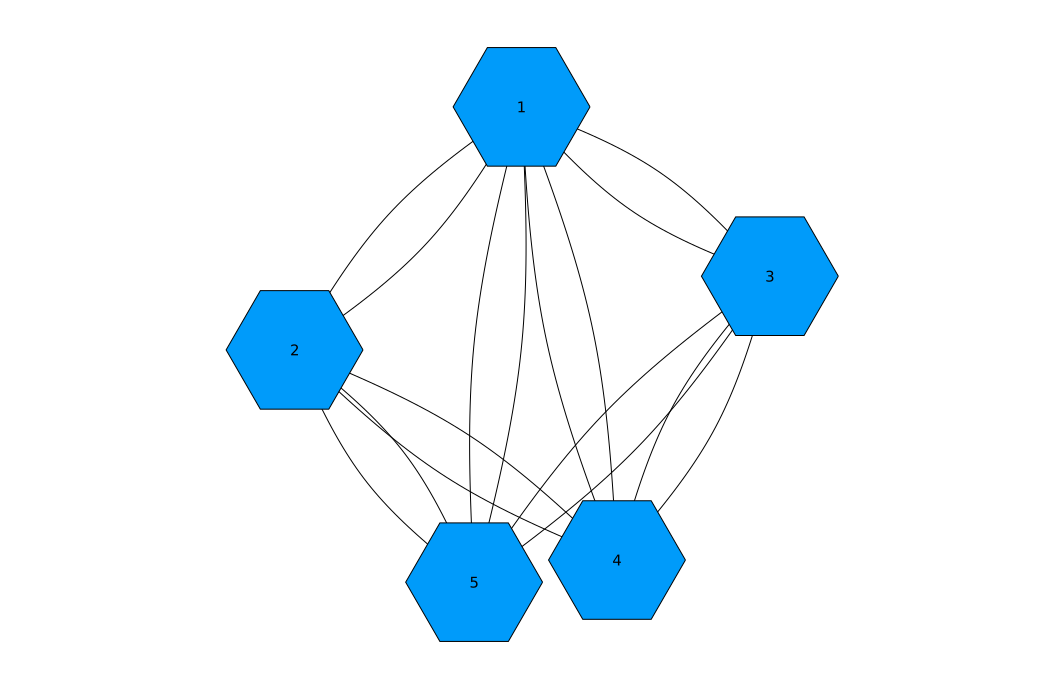
\includegraphics[width=\linewidth]{jl_IBhjS5/generative_2_1.png}

We now define a generative model using the inputs from above.


\begin{lstlisting}
(*@\HLJLn{gen}@*) (*@\HLJLoB{=}@*) (*@\HLJLnf{GenerativePropODE}@*)(*@\HLJLp{(}@*)(*@\HLJLn{x\ensuremath{\_0}}@*)(*@\HLJLp{,}@*) (*@\HLJLnf{fill}@*)(*@\HLJLp{(}@*)(*@\HLJLn{propogate}@*)(*@\HLJLp{,}@*) (*@\HLJLn{n}@*)(*@\HLJLp{),}@*) (*@\HLJLn{p}@*)(*@\HLJLp{,}@*) (*@\HLJLn{g}@*)(*@\HLJLp{,}@*) (*@\HLJLn{\ensuremath{\tau}}@*)(*@\HLJLp{);}@*)
\end{lstlisting}


Using the \texttt{generate} function we can solve this system with the given parameters. This is all done courtesy of \texttt{DifferentialEquations.jl}. Note here that any subtype of \texttt{PropODE} can use the generate method which give inferred models based on real data the ability to project expression into the future. The following is a type diagram for the \texttt{PropODE} so you can see the different models in the works.


\begin{lstlisting}
(*@\HLJLnf{plot}@*)(*@\HLJLp{(}@*)(*@\HLJLn{NeuralGRN}@*)(*@\HLJLoB{.}@*)(*@\HLJLn{PropODE}@*)(*@\HLJLp{,}@*) (*@\HLJLn{method}@*) (*@\HLJLoB{=}@*) (*@\HLJLsc{:tree}@*)(*@\HLJLp{,}@*) (*@\HLJLn{fontsize}@*) (*@\HLJLoB{=}@*) (*@\HLJLni{8}@*)(*@\HLJLp{,}@*) (*@\HLJLn{nodeshape}@*) (*@\HLJLoB{=}@*) (*@\HLJLsc{:rect}@*)(*@\HLJLp{,}@*) (*@\HLJLn{fmt}@*) (*@\HLJLoB{=}@*) (*@\HLJLsc{:svg}@*)(*@\HLJLp{)}@*)
\end{lstlisting}

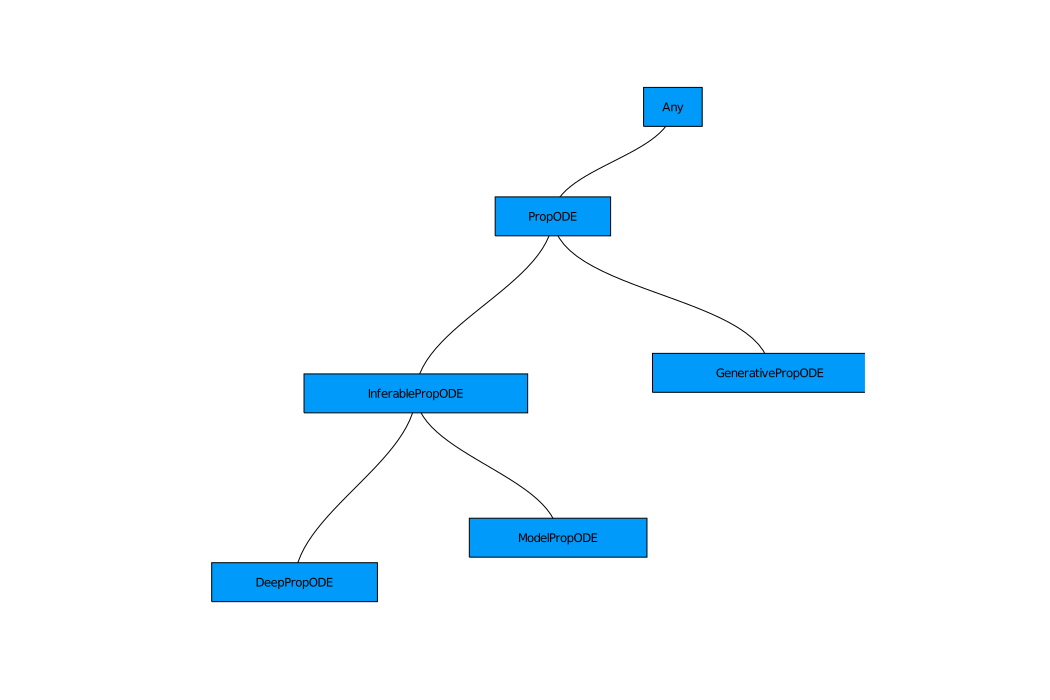
\includegraphics[width=\linewidth]{jl_IBhjS5/generative_4_1.png}

We can run the inference and then plot the resulting data.


\begin{lstlisting}
(*@\HLJLn{results}@*) (*@\HLJLoB{=}@*) (*@\HLJLnf{generate}@*)(*@\HLJLp{(}@*)(*@\HLJLn{gen}@*)(*@\HLJLp{);}@*)
(*@\HLJLnf{plot}@*)(*@\HLJLp{(}@*)(*@\HLJLn{results}@*)(*@\HLJLp{,}@*) (*@\HLJLn{legend}@*) (*@\HLJLoB{=}@*) (*@\HLJLsc{:bottomright}@*)(*@\HLJLp{,}@*) (*@\HLJLn{fmt}@*) (*@\HLJLoB{=}@*) (*@\HLJLsc{:svg}@*)(*@\HLJLp{)}@*)
\end{lstlisting}

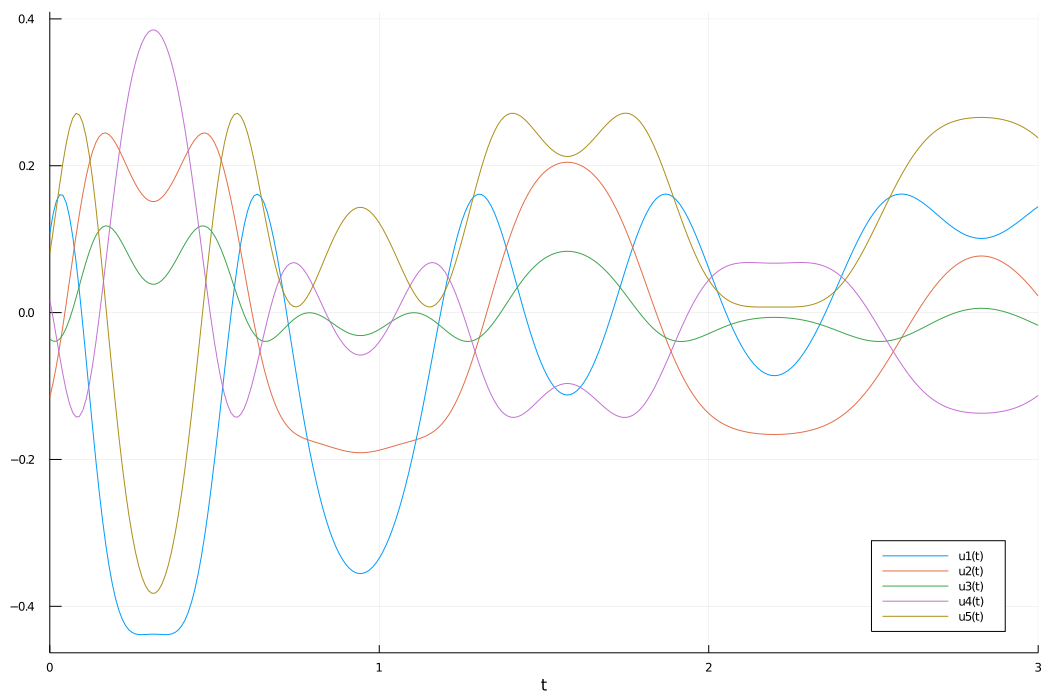
\includegraphics[width=\linewidth]{jl_IBhjS5/generative_5_1.png}


\end{document}
